\documentclass{article}
\usepackage{graphicx}
\usepackage{hyperref}

\title{Assignment 4}
\author{Abbas Khan , Mariia Rybalka , Linara Adilova}
\begin{document}
\maketitle 
    
\section*{Task 4.1 (practical): DNS spoofing}
Source code is in file \textbf{MyDNSSpoofer.py}.
\\
Response for every group member:
\begin{itemize}
\item
Received IP: 254.109.186.165
\\Resolves to user: adilova
\\Associated secret: Waledac
\item 
Received IP: 183.83.20.158
\\Resolves to user: rybalka
\\Associated secret: Whitehat
\item
Received IP: 158.149.246.215
\\Resolves to user: khan
\\Associated secret: Sniffing
\end{itemize}


\section*{Task 4.2 (theoretical): Message Authentication Code (MAC)}
Since each $x_{i}$ is 64 bit , the resultant hash K will also be 64 bit.If a 64-bit hash is used, there are approximately 1.8 x 10$^{19}$ different outputs. If these are all equally probable (the best case), then it would take 'only' approximately 5 billion attempts( 5.1 x 10$^{9}$) to generate a collision using brute force. This value is called birthday bound and for n-bit codes it could be computed as 2$^{n}$/2\cite{birthday_attack}
\section*{Task 4.3 (practical): Diffie-Hellman}
Exploited - man in the middle (details)
\\
Source code is in file \textbf{diffie\_hellman.py}.
\\
Decrypted communication:
\\- Done. Hey, can you tell me the password of your Dridex botnet?
\\- Haha, you are so evil! Ship me 42 euros! :) Just kidding, it is "s00p4doOPas3cReT".
\\- No no! I am a whitehat ;)... thanks and bye!
\\- Bla bla... ;) - bye!

\section*{Task 4.4 (theoretical): TLS Cipher Suites}
\subsection*{TLS\_ECDHE\_RSA\_WITH\_AES\_128\_GCM\_SHA256}
\cite{tls-ref}
\\
In this suite client and server generate pre-master key using Ephemeral Elliptic Curve Diffie-Hellman (ECDHE) and this exchange will be verified using RSA keys. So here RSA is used for Authentication. 
\\
Then package exchange will be processed with 128 bit AES in Galois Counter Mode (AES\_128\_GCM). So this method is used for Encryption.
\\
And for MAC SHA256 is used. It performs both Integrity and Authentication.

\subsection*{TLS\_RSA\_WITH\_RC4\_128\_MD5}
Here pre-master key is generated with RSA - authentication part. Then packages are encrypted with 128 bit Rivest Cipher 4 (RC4\_128) - encryption part. And Mac is created with MD5 - integrity and authentication.

\subsection*{Reasons}
Three reasons why first suite is considered to be more secure than the second one:
\begin{enumerate}
\item First suite provides so called Prefect Forward Secrecy (\cite{pfc}). When client and server use RSA to generate pre-master key, they use server's RSA and server's RSA public key is a part of server certificate and stored for a long time. So if it will be compromised all the previous connections (if somebody will record them) can be decrypted. While with ECDHE keys are generated for every connection and forgot after connection is closed. So attacker would have to break the encryption for every connection separately.
\item RC4 is proved to be insecure with many different vulnerabilities. One of them is described in \cite{rc4-vuln} - statistical weakness, that alows to distinguish between short outputs of RC4 and random strings by analyzing their second bytes. 
\item MD5 hash function compromised by allowing collisions in the output, i.e. there exist another message, not equal to the initial, that will give the same MD5 value. So, the authors of the paper \cite{md5-coll} showed several practical ways of doing it.
\end{enumerate}

\section*{Task 4.5 (practical): Cipher Suites in the Wild}
Script is in file \textbf{ssl\_suits.sh}. Used list of top sites from Alexa Top 500 (\textbf{top\_sites.txt}). Checked ciphersuits are from OpenSSL 1.0.2g. Histogram of usage is depicted in Figure \ref{fig:hist}. Also attached as file \textbf{histogram-suits.png} because of bad readability. Script used for drawing is in file \textbf{ssl\_suites\_hyst.py}

\begin{figure}[h]
    \centering
    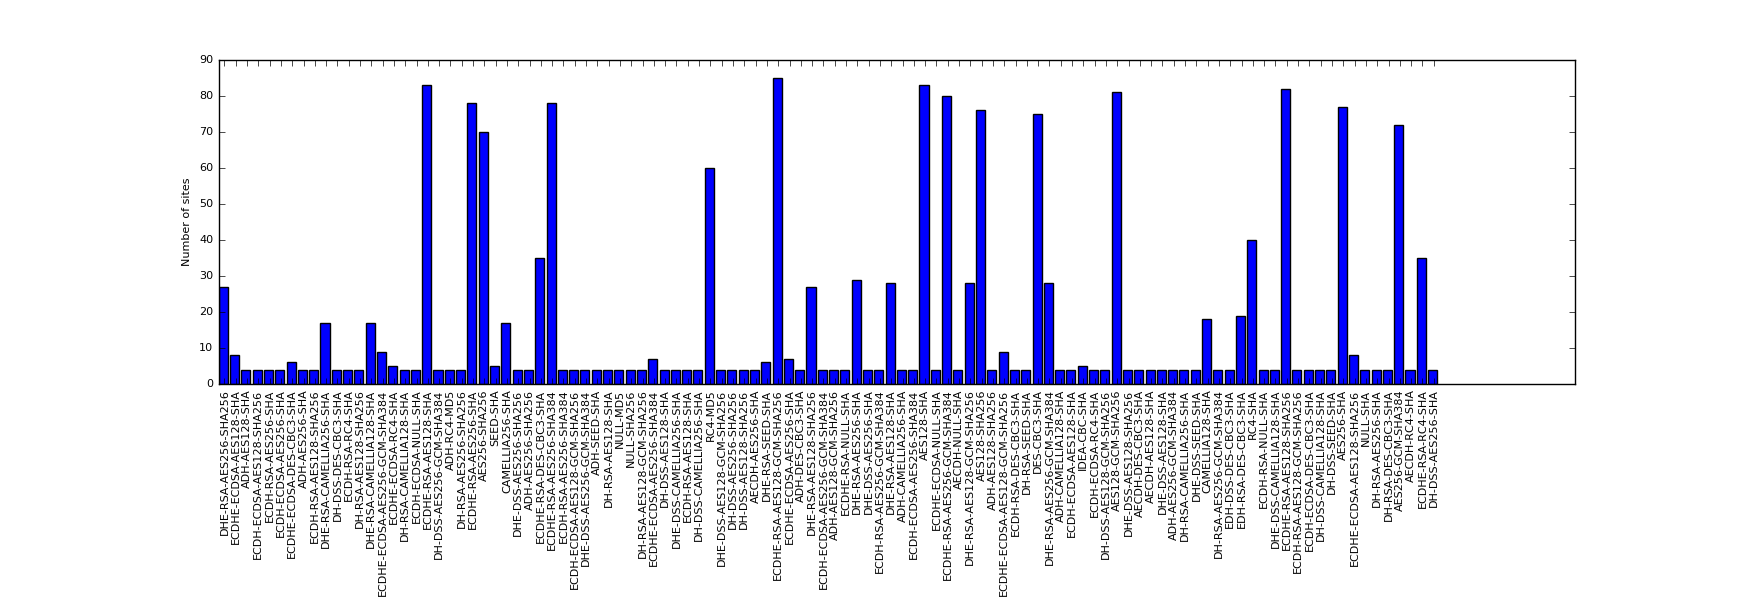
\includegraphics[width=\textwidth]{histogram-suits.png}
    \caption{Histogram of usage of TLS cipher suits}
    \label{fig:hist}
\end{figure}

\begin{thebibliography}{9}

\bibitem{birthday_attack}
\emph{\url{https://en.wikipedia.org/wiki/Birthday_attack}}

\bibitem{tls-ref}
  TLS Elliptic Curve Cipher Suites with SHA-256/384 and AES Galois Counter Mode (GCM)
  \emph{\url{https://tools.ietf.org/html/rfc5289}}
  
\bibitem{pfc}
  Perfect Forward Secrecy
  \emph{\url{https://www.perfectforwardsecrecy.com/}}
  Sponsored by Encryption Chat

\bibitem{md5-coll}
  A Study of the MD5 Attacks: Insights and Improvements
  \emph{\url{http://www.cs.colorado.edu/~jrblack/papers/md5e-full.pdf}}
  J. Black, M.Cochran, T. Highlandy
  
\bibitem{rc4-vuln}
  A Practical Attack on Broadcast RC4
  \emph{\url{http://saluc.engr.uconn.edu/refs/stream_cipher/mantin01attackRC4.pdf}}
  Itsik Mantin and Adi Shamir\\
  Computer Science Department, The Weizmann Institute, Rehovot 76100, Israel

  
\end{thebibliography}

\end{document} 
